\documentclass[aspectratio=169]{beamer}
\usetheme{IITiS}

\usepackage[utf8]{inputenc}
\usepackage{caption}

\title[Kandydatura doktorancka]{Kandydatura do szkoły doktorskiej}
\subtitle{Practical quantum advantage in optimization: hybrid algorithms and classical HPC baselines}
\author{Philipp Hanussek}
\institute{IITiS PAN, Gliwice \\ Promotor: dr hab. inż. Łukasz Pawela}
\date{\today}

\begin{document}

% --- Tytuł ---------------------------------------------------------------
\begin{frame}[plain]
	\titlepage
\end{frame}

% --- Plan prezentacji -----------------------------------------------------
\begin{frame}{Plan prezentacji}
	\tableofcontents
\end{frame}

\section{O mnie}

\begin{frame}
	\dividerpage{O mnie}
\end{frame}

\begin{frame}{Wykształcenie}
	\begin{itemize}
		\item \textbf{Sorbonne Université}, Paryż, Francja \hfill \textit{09/2024 -- 09/2026}
		      \begin{itemize}
			      \item Magister Informatyki
			      \item Kursy: Deep Learning, Parallel Computing using OpenMP, kryptografia (w~tym kwantowa)
		      \end{itemize}
		\item \textbf{FH Aachen}, Akwizgran, Niemcy \hfill \textit{2020 -- 2024}
		      \begin{itemize}
			      \item Licencjat z Informatyki, GPA 3.5/4 (z~wyróżnieniem), top 5\% rocznika (2021, 2022), stypendium za wyniki w~nauce (2023)
			      \item Praca dyplomowa: \textit{Comparison of Factoring Methods on the D-Wave Quantum Annealer}
		      \end{itemize}
	\end{itemize}
\end{frame}

\section{Doświadczenie zawodowe}

\begin{frame}{Doświadczenie zawodowe}
	\begin{itemize}
		\item \textbf{ZKSI}, Polska Akademia Nauk -- IITiS \hfill \textit{2+6 miesiący}
		\item \textbf{Quantum Information Group}, Jülich Supercomputing Centre \hfill \textit{6 miesięcy}
	\end{itemize}
	\vspace{0.6em}
	\begin{block}{Kluczowe osiągnięcia}
		\begin{itemize}
			\item \textit{Quantum-inspired dynamical models on quantum and classical annealers} -- Phys. Rev. Applied (2026), pierwszy autor
			\item \textit{The State of Factoring on Quantum Computers} -- NIC Symposium (2025), współautor
		\end{itemize}
	\end{block}
\end{frame}

\section{Uzasadnienie interesu badawczego}

\begin{frame}
	\dividerpage{\Large Uzasadnienie interesu\\dla tematu badawczego}
\end{frame}

\begin{frame}{Uzasadnienie interesu dla tematu badawczego}
	\begin{itemize}
		\item \textbf{Kontynuacja i~rozszerzenie} -- w~tym na inne komputery kwantowe (poza D-Wave)
		\item \textbf{Opracowanie i~systematyzacja nowych metod}
	\end{itemize}
\end{frame}

\section{Praca magisterska oraz temat badawczy doktoratu}

\begin{frame}
	\dividerpage{\Large Praca magisterska\\oraz temat badawczy doktoratu}
\end{frame}

\begin{frame}{Czym jest D-Wave?}
	\begin{itemize}
		\item Komputer kwantowy typu \textbf{quantum annealer} -- wyspecjalizowane urządzenie do rozwiązywania problemu Isinga
		\item Poszukuje konfiguracji spinów $\widehat\sigma_z^{(i)} \in \{-1,+1\}$ minimalizującej energię układu
	\end{itemize}
	\begin{block}{Hamiltonian Isinga}
		\[
			H_P = \sum_{i=1}^{N} h_i\, \widehat\sigma_z^{(i)} + \sum_{i<j} J_{ij}\, \widehat\sigma_z^{(i)} \widehat\sigma_z^{(j)}
		\]
	\end{block}
\end{frame}

\begin{frame}{Praca licencjacka -- problem faktoryzacji}
	\begin{itemize}
		\item Faktoryzacja liczb całkowitych jako problem optymalizacyjny -- odwzorowanie na problem Isinga rozwiązywalny przez D-Wave
	\end{itemize}
	\begin{block}{Sformułowanie problemu (QUBO)}
		\[
			N = p \cdot q
		\]
		\begin{itemize}
			\item $N$ -- znana liczba całkowita, którą chcemy rozłożyć na czynniki
			\item $p, q$ -- nieznane czynniki (liczby pierwsze), szukane przez solver
		\end{itemize}
	\end{block}
\end{frame}

\begin{frame}{Dynamika czasowa układów few-qubit (QUBO)}
	\begin{columns}[T]
		\begin{column}{0.55\textwidth}
			\textbf{Układ fizyczny:} few-body,zależny od czasu 
			\[
				i\,\partial_t |\psi(t)\rangle = H(t)\,|\psi(t)\rangle
			\]
			\vspace{0.3cm}
			\begin{itemize}
				\item Kodowanie: stan historii równoległej w~czasie
				      $|\Psi\rangle = \sum_n |t_n\rangle \otimes |\psi(t_n)\rangle$
				\item \textbf{Cel:} trajektoria $|\psi(t)\rangle$ w~każdym kroku czasowym
			\end{itemize}
		\end{column}
		\begin{column}{0.45\textwidth}
			\centering
			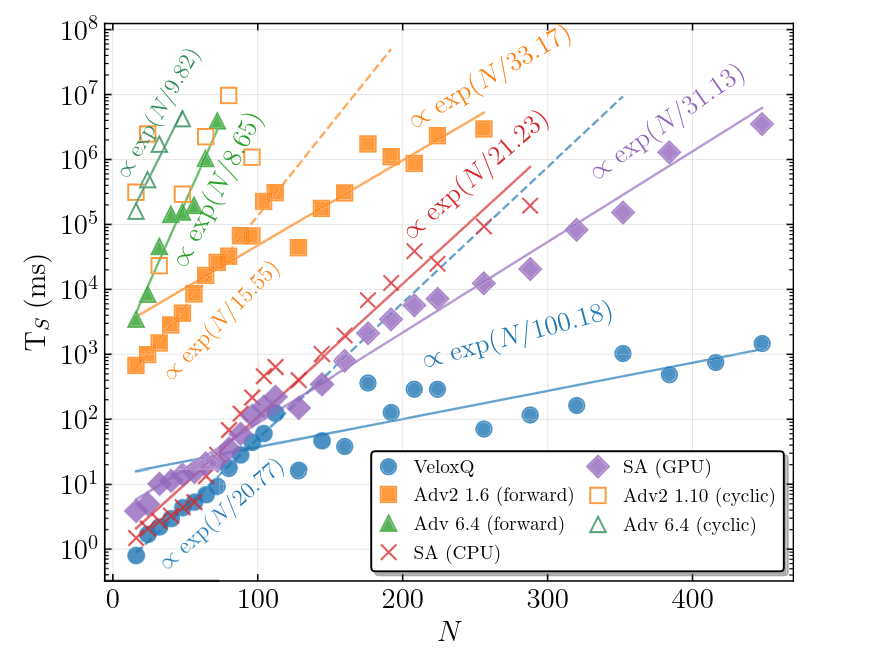
\includegraphics[width=\textwidth]{figures/tts_scaling.png}
			\captionof{figure}{Skalowanie czasu rozwiązania $T_s$ vs.\ rozmiar problemu $N$}
		\end{column}
	\end{columns}
\end{frame}

\begin{frame}{Stan podstawowy TFIM poprzez RBM / VMC}
	\begin{columns}[T]
		\begin{column}{0.55\textwidth}
			\textbf{Układ fizyczny:} statyczny, niezależny od czasu układ wielociałowy na~sieci
			\[
				H = -\sum_{\langle i,j\rangle} \sigma_i^z \sigma_j^z \;-\; h \sum_i \sigma_i^x
			\]
			\vspace{0.3cm}
			\begin{itemize}
				\item Ansatz: funkcja falowa RBM $\Psi(v)$
				\item porównanie $TT_\epsilon$ na klasycznych metodach (GPU, FPGA) i komputerach kwantowych
			\end{itemize}
		\end{column}
		\begin{column}{0.45\textwidth}
			\centering
			
\includegraphics[height=4.3cm,keepaspectratio]{figures/embedding_full_zephyr.pdf}
			\captionof{figure}{Osadzenie problemu na topologii Zephyr}
		\end{column}
	\end{columns}
\end{frame}

\begin{frame}{Szerszy kontekst doktoratu}
	\begin{itemize}
		\item Rzetelny benchmarking: quantum annealing vs.\ klasyczne HPC
		\item Pytanie: czy realna jest bliskoterminowa przewaga kwantowa?
	\end{itemize}
\end{frame}

% --- Zakończenie -----------------------------------------------------------
\begin{frame}
	\dividerpage{Dziękuję\\[0.4em]\LARGE\normalfont Pytania?}
\end{frame}

\begin{frame}{Kontakt}
	\centering
	\iitislogo{0.3}\\[1em]
	Philipp Hanussek \\
	\url{hanup@mailbox.org}
\end{frame}

\end{document}
